\documentclass[tikz,border=2mm]{standalone}
\usepackage{mathptmx} % Matches the serif font from the image

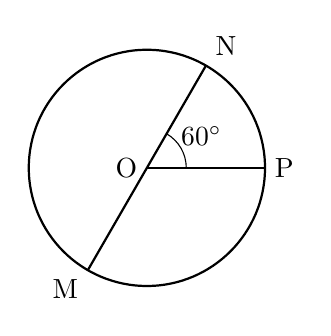
\begin{tikzpicture}[scale=1]
    % Define the radius
    \def\R{1.5cm}

    % Define Coordinates
    \coordinate (O) at (0,0);
    \coordinate (P) at (0:\R);    % 0 degrees (Right)
    \coordinate (N) at (60:\R);   % 60 degrees
    \coordinate (M) at (240:\R);  % 60 + 180 = 240 degrees (Opposite N)

    % 1. Draw the Circle
    \draw[thick] (O) circle (\R);

    % 2. Draw the Lines
    \draw[thick] (M) -- (N); % The diameter MN
    \draw[thick] (O) -- (P); % The radius OP

    % 3. Draw the Angle Arc
    % Arc starts at 0 deg, ends at 60 deg, radius 0.5cm
    \draw[thin] (0.5,0) arc (0:60:0.5);
    \node at (30:0.8) {$60^\circ$};

    % 4. Add Labels
    \node[left] at (O) {O};
    \node[above right] at (N) {N};
    \node[right] at (P) {P};
    \node[below left] at (M) {M};

\end{tikzpicture}